\chapter{Extraction of spin correlation}

\section{Likelihood Fit}
\label{sec:extraction}

We extract the amount of spin correlation in the data in several variables by fitting templates using a binnned maximum likelihood method. 



\section{Systematic Uncertainties}
\label{sec:systematics}

The use of Monte Carlo simulations in this analysis presents an inherent problem. Though the degree to which these samples accurately reflect the true physics processes that they simulate is impressive, they are not perfect. A systemic disparity occurs between our assumption; the rates and shapes of the signal and backgrounds distributions, and the observed data. This is described as a ``systematic'' uncertainty. The effect of these systematic uncertainties, or more simpliy put the effect of the difference between our simulation and truth, must be quantified.

Pseudo experiments are used to estimate the effect of a source of uncertainty. In order to negate statistical effects in the fit, many pseudo experiments are performed, each time varying the shifted template poissonly. The step by step procedure is described below:
 
\begin{enumerate}
	\item Fit the nominal templates to the data and obtain $f_{SM}^{nominal}$.
	\item Generate new spin and no spin templates, with a systematic shift 'X' included.
	\item Construct \textit{pseudo data} by mixing the shifted spin and shifted no spin templates to the same degree $f_{SM}^{nominal}$. Poisson vary each bin, using the bin content as the mean.
	\item Refit the nominal templates to this new \textit{pseudo data} and obtain $f_{SM}^{X~shifted}$.
	\item Repeat 2-4 many times and fit the resulting distribution with a gaussian curve (illustrated in figure \ref{fig:syst_gaussian}). Extract the mean to obtain $f_{SM}^{X}$.
	\item Take $f_{SM}^{nominal}$ - $f_{SM}^{X}$ as the systematic shift uncertainty.
\end{enumerate}

For this analysis we quote the degree to which the uncertainty may effect the result within onc confidence interval ($1\sigma$ deviation). In the majority of cases, a parameter is shifted within some estimated uncertainty and the extraction of spin correlation is reperformed. The difference between the nominal fit and the systematic shifted fit is taken to be the $1\sigma$ uncertainty associated with that source of systematic. In other cases a unique prescription may be used and are detailed case by case in the following section.

\begin{figure}[htbp]
\begin{center}
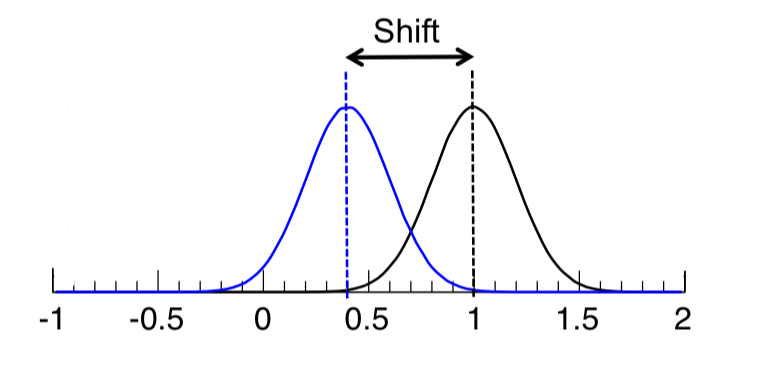
\includegraphics[width=100mm]{f/GaussianFigure}
\end{center}
\caption{Illustration of systematic estimation procedure. The caussian curve generated by the systemati shifted pseudo experiments is showin in blue, the nominal fit is shown in black}
\label{fig:syst_gaussian}
\end{figure}

Each source of systematic uncertainty is assumed to be uncorrelated and for the total systematic uncertainty all of the individual sources are added in quadrature. In reality some correlations do exists, however steps are taken to reduce the correlation in those cases. 

We give an overview over all sources of systematic uncertainties that we consider and the methods by which they are estimated. For simplicity we categorise systematic uncertainties into two types: 
\begin{itemize}
	\item ``Normalisation uncertaintines'': which only effect the rate of a particular background or signal sample 
	\item ``Shape changing systemaitcs'': which effect the shape of the variable of interest, independent of its normalisation. 
\end{itemize}
Normalisation uncertainties typically have a small effect on the extracted spin correlation as the normalisation of the signal tmplates is allowed to float in the likelihood fit (i.e. the floating of the \ttbar\ cross section described in section \ref{sec:extraction}. Shape changing uncertainties are the dominant form of uncertainty in the analysis and can have a marked impact on the spin correlation.

\vspace{5mm}
\noindent
\textbf{Luminosity:}
\begin{itemize} 
     \item For data taken in the 7TeV LHC running period, the Luminosity uncertainty is taken to be a flat uncertainty of $\pm1.8$~\% on the normalisation of the data, established primarily through van-de-meer scans performed during data taking, and comparisons with the CMS detector [Luminosity Reference]. The systematic uncertainty is estimated by varing the normalisation of both the signal and background samples simultaneously, up and down by this value.
\end{itemize}

\vspace{5mm}
\noindent
\textbf{Electrons:}
\begin{itemize}
    \item Energy Scale: All electrons are corrected for electron energy scale by default in the Monte Carlo. To estimate the systematic uncertainty this energy scale is shifted by $\pm 1\sigma$~ of the uncertainty from the energy scale estimation procedure, in addition to the decault scaling. 
    \item Trigger Scale Factor: To estimate the uncertainty on the scale factor associated with trigger moddeling, the scale factors are varied by $\pm 1\sigma$~ from the default scale factor.
    \item Energy Resolution: The Monte Carlo is smeared by default to correct for the difference in the modelling of electron energy resoluton with the data. Additional smearing is performed to estimate the uncertainty.
\end{itemize}

\vspace{5mm}
\noindent
\textbf{Muons:}
\begin{itemize}
    \item Momentum Shift: There are two possible sources of muon momentum uncertainty, those from the muon spectrometer (MS) and those from the inner detector (ID). The muon momentum is shifted by $\pm~1~\sigma$ in the MS and ID independently. The largest and smallest shift are averaged to provide the uncertainty. Correlations between these parameters are accounted for.
    \item Resolution: The Monte Carlo is smeared by default to correct for the difference in energy resoluton with the data. Additional smearing is performed to estimate the uncertainty.
    \item Momentum Scale: To estimate the effect of muon momentum scaling in the MC, this is disabled and the fit reperformed. The result is then symmeterised and taken as the systematic shift.
\end{itemize}

\vspace{5mm}
\noindent
\textbf{Jets:}
Jets represent one of the most difficult physical object to moddel correctly in Monte Carlo and as such have a large number of sources of systematic uncertainty. 
\begin{itemize}
    \item Jet Energy Scale: A total of 61 sources of systematic uncertainty exist in relation to Jet Energy Scale. Fortunately, many of these are correlated and it is possible to fully cover the uncertainty using 16, uncorrelated variations.
	\begin{enumerate}
	\item JES Component 1
	\item JES Component 2
	\item JES Component 3
	\item JES Component 4
	\item JES Component 5
	\item JES Component 6
	\item JES Component 7
	\item JES Component 8
	\item JES Component 9	
	\item JES Component 10
	\item JES Component 11	
	\item JES Component 12
	\item JES Component 13	
	\item \textit{Falvour Response} - Uncertainty associated with the flavour composition of each jet.
	\item \textit{B-JES} - Energy scale associated with jets tagged with b flavour.
	\end{enumerate}	
    \item Energy Resolution: Jets energies are smeared within uncertainties derived from resolution measurements over the full 2011 data set. 
    \item Reconstruction Efficiency: The efficificieny to reconstruct jets is not 100\% and not identical between data and Monte Carlo. In order to estimate the effect of this efficiecny, jets are randomly dropped from the nominal sample and the spin correlation re-extracted within an efficiency rage derived from data. This shift between this sample and the nominal is symmeterised and taken as the uncertianty.
\end{itemize}

\vspace{5mm}
\noindent
\textbf{MET:}
\begin{itemize}
    \item Pileup: In order to estimate the effect of pileup on MET, the values for MET are scaled up and down by a 6.6\% uncertainty. 
    \item Soft Jet - Cell Out Correction: The systematics due to energy in calorimeter cells not associated to a physics object ('Cell out') and soft jets used in the calculation of the missing ET are 100\% correlated and evaluated together. 
\end{itemize}

\vspace{5mm} 
\noindent
\textbf{Generator Uncertainties:}
\begin{itemize}
    \item Choice of Generator: Two generators are available at ATLAS to simulate \ttbar\ events at next to leading order, MC@NLO and POWHEG. In order to estiumate the uncertainty on the choice of generator, the fit results for both are compared and taken as an uncertainty. In order to isolate only the generator differences, both are interfaced to HERWIG to perform showering. 

    \item Parton Shower / Framentation model: 

    \item ISR / FSR: The effect of initial state and final state radiation is estimated by taking two ACER MC samples, with the same matrix elements, and interfacing them with Pythia to perform showering. The amount of showering is scaled up and down to simulate more initial and final state radiation simultaneously. The systematic shift is defined as half of the difference in the fits of these two samples. 

    \item Template Statistics: The effect of limited template statistics in the signal MC is estimated by poisson fluxuating the standard model template by the number of entries in each bin (as opposed to the noninal statistical uncertainty where the bins are poisson fluctuated by the number of data entries in each bin). The result is then fitted to the original templates to obtain the systematic shift. 
\end{itemize}

\vspace{5mm}
\noindent
\textbf{PDF}
In order to investigate the effect of the choice of PDF used in the analysis (in this case CTEQ6.6) a weight is assigned to each event and the analysis repeated. 
\begin{itemize}
  \item Intra PDF Uncertainty:
  \item Inter PDF Uncertainty:
\end{itemize}

\vspace{5mm}

\noindent
\textbf{Fake Leptons:}
The uncertainty due to mis-identified leptons is different depending on lepton flavour, and so each are measured seperately (and combined in quadrature in the case of the \emu channel). 

\begin{itemize}
    \item Electrons: For mis-identified electrons the dominant uncertainty is due to the different sources of misidentification, or 'flavour fraction'. This predominantly effects the fake efficiency used in the matrix method and so the flavour fractions are varied, resulting in a shift up in the fake efficiency and a shift down. There is also a small contribution to the real efficiency is are also shifted up and down. All four shifts are treated independently, with the largest shift taken as the uncertainty.
    \item Muons: The dominant uncertainty for the muon fake rate is the method used to estimate them. For the uncertainty, the difference of the weights of the two methods is taken (rather than the average as is taken in the nominal case) and the resulting estimate is normalised to the nominal fake normalisation. The muon contribution is therefore purely a shape changing one.
\end{itemize}

\vspace{5mm}
\noindent
\textbf{Monte Carlo Backgrounds:}
\begin{itemize}
    \item Single top normalisation: The systematic uncertainties associated with the single top monte carlo are derived from theory uncertainties and are different for each production channel. 
    \item Diboson normalisation: The uncertainty of the normalisation of the diboson monte carlo shapes is determened individually for the WW, WZ and ZZ channels. For the WZ and ZZ channels, a flat uncertainty of $\pm$5\% is applied. For the WW channel and additional uncertainty of 11.52\% is applied due to the inclusion of additional jets in the WW sample that have not come from the hard process. 
    \item DY background: The systematic uncertainty on the data-drive Drell-Yan estimate is derived by varying the missing energy requirement used to define the control region by $�5 GeV$. The largest difference is taken and the uncertainty is symmeterised (why?). In addition the statistical, Jet Energy Scale, Lepton Energy Scale and Lepton Energy resolution uncertainties are recalculated and added in quadrature for this uncertainty. 
    \item ($Z\rightarrow\tau\tau$): A flat uncertainty of 4\% is applied with an additional 24\% uncertainty for each final state jet in the selection (see Diboson normalisation) of 11.52\%.
\end{itemize}

\begin{table}[htbp]

\footnotesize
\begin{center}
   \begin{tabular}{|c|c|c|c|c|}
   \hline
   \textbf{$\Delta\phi$~6 bins}               &  ee &mumu &emu&all\\
   \hline
   $JES 0$                             &  +0.006   / +0.018   & +0.005   / +0.020   & +0.006   / +0.011   & -0.001   / +0.006   \\
   $JES 1$                             &  - 0.000   / +0.052   & -0.010   / +0.011   & -0.002   / +0.016   & -0.013   / +0.010   \\
   $JES 2$                             &  +0.006   / +0.013   & +0.008   / +0.008   & +0.007   / +0.009   & +0.001   / +0.003   \\
   $JES 3$                             &  +0.001   / +0.000   & +0.016   / +0.010   & +0.011   / +0.008   & +0.001   / +0.003   \\
   $JES 4$                             &  +0.004   / +0.001   & +0.012   / +0.010   & +0.008   / +0.010   & +0.000    / +0.001   \\
   $JES 5$                             &  -0.003   / +0.015   & +0.005   / +0.009   & +0.008   / +0.011   & +0.002   / +0.003   \\
   $JES 6$                             &  +0.004   / +0.021   & +0.011   / +0.013   & +0.009   / +0.009   & +0.000    / +0.004   \\
   $JES 7$                             &  +0.013   / +0.035   & +0.001   / +0.028   & +0.007   / +0.014   & +0.002   / +0.008   \\
   $JES 8$                             &  +0.000    / +0.000    & +0.012   / +0.012   & +0.008   / +0.008   & +0.001   / +0.001   \\
   $JES 9$                             &  -0.008   / +0.010   & -0.010   / +0.005   & +0.004   / +0.007   & -0.011   / -0.001   \\
   $JES {10}$                          &  +0.034   / +0.011   & +0.005   / +0.011   & +0.010   / +0.008   & +0.005   / +0.001   \\
   $JES {11}$                          &  +0.025   / +0.025   & -0.011   / -0.002   & +0.002   / +0.014   & -0.010   / +0.007   \\
   $JES {12}$                          &  -0.015   / +0.020   & +0.005   / +0.004   & -0.001   / +0.011   & -0.006   / +0.007   \\
   $JES {13}$                          &  +0.013   / +0.029   & -0.015   / -0.002   & +0.002   / +0.013   & -0.011   / +0.004   \\
   $JES {14}$                          &  +0.013   / +0.036   & -0.005   / +0.005   & +0.010   / +0.010   & -0.002   / +0.002   \\
   $JES {15}$                          &  -0.015   / +0.031   & -0.003   / +0.017   & +0.005   / +0.013   & -0.003   / +0.006   \\
   \hline
   JES Total                             &  +0.054   / -0.097   & +0.037   / -0.050   & +0.028   / -0.044   & +0.024   / -0.020   \\
   Jet Vertex Fraction                   &  +0.000    / +0.000    & +0.012   / +0.012   & +0.008   / +0.008   & +0.001   / +0.001   \\
   Jet Energy Resolution                 &  +0.013   / +0.013   & +0.007   / +0.007   & +0.002   / +0.002   & +0.005   / +0.005   \\
   Jet Reconstruction Eff                &  +0.011   / +0.011   & +0.004   / +0.004   & +0.013   / +0.013   & +0.004   / +0.004   \\
   \hline
   \textbf{JET Total}                    &  +0.057   / -0.098   & +0.040   / -0.052   & +0.032   / -0.046   & +0.025   / -0.021   \\
   \hline
   Electron Energy Smearing              &  +0.024   / +0.020   & +0.013   / +0.012   & +0.009   / +0.008   & +0.003   / +0.002   \\
   Electron Energy Scale                 &  +0.026   / -0.010   & +0.024   / +0.014   & -0.021   / +0.007   & -0.013   / +0.000    \\
   Scale Factor (ee)                     &  -0.013   / -0.025   &         &      & -0.004   / +0.002   \\
   Scale Factor (mumu)                   &       & +0.002   / -0.002   &     & -0.001   / -0.001   \\
   Scale Factor (emu)                    &       &     & +0.008   / +0.007   & +0.002   / -0.004   \\
   Muon Momentum Scale offset            &  +0.005   / +0.005   & +0.007   / +0.007   & +0.011   / +0.011   & +0.006   / +0.006   \\
   Muon Momentum Smearing                &  +0.063   / +0.063   & +0.009   / +0.009   & +0.026   / +0.026   & +0.019   / +0.019   \\
   \hline
   \textbf{LEPTON Total}                 &  +0.073   / -0.071   & +0.029   / -0.022   & +0.037   / -0.031   & +0.024   / -0.020   \\
   \hline
   Muon Fake Shape                       &        & +0.014   / +0.014   & +0.051   / +0.051   & +0.013   / +0.013   \\
   Fake Normalisation                    &  -0.036   / +0.049   & +0.012   / +0.008   & -0.006   / +0.026   & -0.013   / +0.016   \\
   Electron eff Real                     &  +0.002   / +0.059   &       & +0.006   / +0.015   & -0.004   / +0.013   \\
   Electron eff Fake                     &  -0.036   / +0.065   &      & -0.019   / +0.028   & -0.022   / +0.019   \\
   \hline
   \textbf{Fake Total}                   &  +0.051   / -0.100   & +0.019   / -0.017   & +0.055   / -0.065   & +0.029   / -0.031   \\
   \hline
   MET pileup                            &  -0.006   / -0.001   & +0.024   / -0.000   & +0.008   / +0.008   & +0.003   / -0.002   \\
   MET soft cell out                     &  +0.012   / -0.008   & +0.030   / -0.005   & +0.008   / +0.008   & +0.005   / -0.003   \\
   \hline
   \textbf{MET Total}                    &  +0.013   / -0.008   & +0.038   / -0.005   & +0.011   / -0.011   & +0.006   / -0.004   \\
   \hline
   Single Top normalisation              &  +0.009   / +0.013   & +0.008   / +0.011   & +0.008   / +0.011   & +0.002   / +0.002   \\
   Ztautau normalisation                 &  +0.035   / -0.013   & +0.035   / -0.011   & +0.013   / +0.001   & +0.013   / -0.013   \\
   Diboson normalisation (WW)            &  -0.003   / +0.020   & +0.014   / +0.009   & +0.009   / +0.010   & -0.001   / +0.004   \\
   Diboson normalisation (WZ)            &  +0.000   / +0.002   & +0.016   / +0.013   & +0.009   / +0.009   & +0.002   / +0.001   \\
   Diboson normalisation (ZZ)            &  -0.001   / -0.000   & +0.013   / +0.011   & +0.009   / +0.008   & +0.000   / +0.001   \\
   \hline
   \textbf{MC Background Total}          &  +0.036   / -0.027   & +0.044   / -0.024   & +0.022   / -0.019   & +0.013   / -0.014   \\
   \hline
   Template Statistics                   &  +0.049   / +0.049   & +0.106   / +0.106   & +0.096   / +0.096   & +0.506   / +0.506   \\
   Luminosity                            &  +0.014   / +0.002   & +0.019   / +0.001   & +0.009   / +0.009   & +0.000   / -0.003   \\
   ISR/FSR                               &  +0.140   / +0.140   & +0.153   / +0.153   & +0.080   / +0.080   & +0.092   / +0.092   \\
   PS and Fragmentation                  &  +0.202   / +0.202   & +0.174   / +0.174   & +0.071   / +0.071   & +0.099   / +0.099   \\
   NLO Generator                         &  +0.229   / +0.229   & +0.152   / +0.152   & +0.091   / +0.091   & +0.109   / +0.109   \\
   \hline
   \textbf{Generator Total}              &  +0.340   / -0.340   & +0.297   / -0.297   & +0.170   / -0.170   & +0.535   / -0.535   \\
   \hline
   \hline
   \textbf{Total Uncertainty (syst)}     &  +0.358   / -0.376   & +0.305   / -0.303   & +0.187   / -0.192   & +0.537   / -0.537   \\
   \textbf{Total Uncertainty (stat)}     &  +0.314   / -0.314   & +0.166   / -0.166   & +0.097   / -0.097   & +0.085   / -0.085   \\
   \hline
   \end{tabular}
 
   \end{center}
 \end{table}

 \begin{table}[htbp]
\footnotesize
   \begin{center}
   \begin{tabular}{|c|c|c|c|c|}
   \hline
     \textbf{$\Delta\phi$ 10 bins}              &  ee &mumu &emu&all\\
   \hline
   $JES 0$                             &  +0.010   / +0.001   & -0.001   / +0.018   & -0.009   / -0.002   & -0.006   / +0.002   \\
   $JES 1$                             &  -0.022   / +0.010   & -0.017   / -0.002   & -0.014   / +0.002   & -0.016   / +0.006   \\
   $JES 2$                             &  -0.005   / -0.010   & -0.004   / -0.004   & -0.007   / -0.003   & -0.004   / -0.002   \\
   $JES 3$                             &  -0.002   / +0.001   & +0.004   / +0.001   & -0.003   / -0.004   & -0.002   / -0.005   \\
   $JES 4$                             &  +0.006   / +0.003   & +0.003   / +0.002   & -0.005   / -0.004   & -0.004   / -0.004   \\
   $JES 5$                             &  +0.005   / -0.005   & -0.009   / +0.004   & -0.006   / -0.003   & -0.007   / -0.002   \\
   $JES 6$                             &  +0.003   / -0.008   & -0.006   / +0.005   & -0.006   / -0.003   & -0.005   / -0.002   \\
   $JES 7$                             &  +0.023   / +0.001   & -0.008   / +0.016   & -0.005   / +0.002   & -0.004   / +0.002   \\
   $JES 8$                             &  +0.003   / +0.003   & +0.002   / +0.002   & -0.005   / -0.005   & -0.004   / -0.004   \\
   $JES 9$                             &  +0.016   / -0.005   & -0.019   / -0.006   & -0.012   / -0.006   & -0.011   / -0.006   \\
   $JES {10}$                          &  -0.003   / -0.004   & -0.010   / -0.007   & -0.002   / -0.006   & -0.000   / -0.006   \\
   $JES {11}$                          &  -0.006   / +0.015   & -0.026   / -0.022   & -0.012   / +0.003   & -0.009   / +0.003   \\
   $JES {12}$                          &  -0.025   / +0.008   & -0.001   / +0.003   & -0.014   / -0.000   & -0.011   / +0.006   \\
   $JES {13}$                          &  -0.010   / -0.002   & -0.023   / -0.018   & -0.013   / +0.001   & -0.012   / +0.003   \\
   $JES {14}$                          &  -0.003   / +0.005   & -0.016   / -0.004   & -0.004   / -0.002   & -0.006   / -0.002   \\
   $JES {15}$                          &  -0.018   / -0.000   & -0.002   / +0.007   & -0.012   / -0.000   & -0.011   / +0.004   \\
   \hline
   JES Total                             &  +0.051   / -0.026   & +0.050   / -0.040   & +0.037   / -0.013   & +0.032   / -0.016   \\
   Jet Vertex Fraction                   &  +0.003   / +0.003   & +0.002   / +0.002   & -0.005   / -0.005   & -0.004   / -0.004   \\
   Jet Energy Resolution                 &  +0.013   / +0.013   & +0.026   / +0.026   & +0.004   / +0.004   & +0.005   / +0.005   \\
   Jet Reconstruction Eff                &  +0.012   / +0.012   & +0.015   / +0.015   & +0.001   / +0.001   & +0.001   / +0.001   \\
   \hline
   \textbf{JET Total}                    &  +0.054   / -0.031   & +0.058   / -0.050   & +0.037   / -0.015   & +0.033   / -0.017   \\
   \hline
   Electron Energy Smearing              &  +0.013   / -0.003   & +0.002   / +0.002   & -0.003   / -0.005   & +0.002   / -0.002   \\
   Electron Energy Scale                 &  +0.038   / -0.024   & +0.017   / +0.003   & -0.028   / -0.007   & -0.007   / -0.005   \\
   Scale Factor (ee)                     &  -0.027   / -0.038   & +0.000   / +0.000   & +0.000   / +0.000   & -0.003   / -0.002   \\
   Scale Factor (mumu)                   &  +0.000   / +0.000   & -0.012   / -0.016   & +0.000   / +0.000   & -0.007   / -0.007   \\
   Scale Factor (emu)                    &  +0.000   / +0.000   & +0.000   / +0.000   & -0.006   / -0.007   & -0.005   / -0.008   \\
   Muon Momentum Scale offset            &  +0.001   / +0.001   & +0.001   / +0.001   & +0.000   / +0.000   & +0.000   / +0.000   \\
   Muon Momentum Smearing                &  +0.044   / +0.044   & +0.007   / +0.007   & +0.030   / +0.030   & +0.020   / +0.020   \\
   \hline
   \textbf{LEPTON Total}                 &  +0.066   / -0.063   & +0.022   / -0.018   & +0.041   / -0.032   & +0.023   / -0.023   \\
   \hline
   Muon Fake Shape                       &  +0.000   / +0.000   & +0.003   / +0.003   & +0.031   / +0.031   & +0.009   / +0.009   \\
   Fake Normalisation                    &  -0.037   / +0.023   & -0.001   / -0.001   & -0.018   / +0.010   & -0.011   / +0.009   \\
   Electron eff Real                     &  -0.030   / +0.025   & +0.000   / +0.000   & -0.006   / +0.005   & -0.005   / +0.007   \\
   Electron eff Fake                     &  +0.027   / +0.010   & +0.000   / +0.000   & -0.028   / +0.011   & -0.016   / +0.010   \\
   \hline
   \textbf{Fake Total}                   &  +0.055   / -0.036   & +0.003   / -0.003   & +0.045   / -0.035   & +0.022   / -0.018   \\
   \hline
   MET pileup                            &  -0.009   / -0.015   & +0.012   / -0.005   & -0.005   / -0.005   & +0.003   / -0.003   \\
   MET soft cell out                     &  -0.012   / -0.031   & +0.015   / -0.012   & -0.005   / -0.005   & +0.005   / -0.003   \\
   \hline
   \textbf{MET Total}                    &  +0.015   / -0.034   & +0.019   / -0.013   & +0.006   / -0.006   & +0.006   / -0.005   \\
   \hline
   Single Top normalisation              &  -0.008   / -0.009   & -0.002   / +0.002   & -0.003   / -0.003   & -0.004   / -0.001   \\
   Ztautau normalisation                 &  +0.026   / -0.041   & +0.019   / -0.017   & +0.004   / -0.011   & +0.010   / -0.016   \\
   Diboson normalisation (WW)            &  -0.016   / -0.011   & -0.003   / +0.006   & -0.006   / -0.002   & -0.005   / +0.001   \\
   Diboson normalisation (WZ)            &  -0.005   / +0.003   & +0.003   / +0.004   & -0.001   / -0.004   & -0.005   / -0.005   \\
   Diboson normalisation (ZZ)            &  -0.002   / +0.002   & +0.002   / +0.002   & -0.004   / -0.005   & -0.004   / -0.004   \\
   \hline
   \textbf{MC Background Total}          &  +0.032   / -0.044   & +0.020   / -0.019   & +0.009   / -0.013   & +0.013   / -0.017   \\
   \hline
   Template Statistics                   &  +0.145   / +0.145   & +0.091   / +0.091   & +0.082   / +0.082   & +0.310   / +0.310   \\
   Luminosity                            &  -0.015   / -0.006   & +0.011   / -0.003   & -0.003   / -0.003   & -0.002   / -0.005   \\
   ISR/FSR                               &  +0.134   / +0.134   & +0.133   / +0.133   & +0.065   / +0.065   & +0.089   / +0.089   \\
   PS and Fragmentation                  &  +0.170   / +0.170   & +0.178   / +0.178   & +0.063   / +0.063   & +0.090   / +0.090   \\
   NLO Generator                         &  +0.211   / +0.211   & +0.151   / +0.151   & +0.088   / +0.088   & +0.104   / +0.104   \\
   \hline
   \textbf{Generator Total}              &  +0.336   / -0.336   & +0.284   / -0.284   & +0.151   / -0.151   & +0.351   / -0.351   \\
   \hline
   \hline
   \textbf{Total Uncertainty (syst)}     &  +0.352   / -0.347   & +0.291   / -0.289   & +0.167   / -0.159   & +0.354   / -0.353   \\
   \textbf{Total Uncertainty (stat)}     &  +0.321   / -0.321   & +0.176   / -0.176   & +0.104   / -0.104   & +0.087   / -0.087   \\
   \hline
   \end{tabular}
 
   \end{center}
 \end{table}

 \begin{table}[htbp]
\footnotesize
   \begin{center}
   \begin{tabular}{|c|c|c|c|c|}
   \hline
     \textbf{coscos op}        &  ee &mumu &emu&all\\
   \hline
   $JES 0$                             &  -0.047   / -0.088   & -0.007   / +0.012   & +0.000   / -0.042   & -0.005   / -0.026   \\
   $JES 1$                             &  -0.016   / -0.007   & -0.023   / +0.020   & -0.026   / -0.013   & -0.021   / -0.001   \\
   $JES 2$                             &  +0.032   / +0.020   & -0.082   / -0.014   & -0.002   / +0.019   & -0.002   / +0.031   \\
   $JES 3$                             &  -0.025   / +0.051   & -0.031   / -0.019   & +0.012   / -0.004   & +0.007   / +0.009   \\
   $JES 4$                             &  +0.032   / +0.030   & +0.031   / +0.010   & -0.017   / +0.015   & +0.010   / +0.022   \\
   $JES 5$                             &  +0.008   / -0.009   & +0.024   / +0.028   & -0.010   / -0.019   & +0.006   / -0.003   \\
   $JES 6$                             &  -0.044   / +0.018   & +0.011   / +0.022   & -0.028   / -0.025   & -0.017   / -0.006   \\
   $JES 7$                             &  -0.018   / -0.042   & -0.007   / +0.002   & +0.022   / -0.015   & +0.018   / -0.004   \\
   $JES 8$                             &  +0.019   / +0.019   & -0.007   / -0.007   & -0.009   / -0.009   & +0.000   / +0.000   \\
   $JES 9$                             &  +0.000   / -0.013   & +0.008   / +0.003   & -0.005   / +0.003   & +0.009   / +0.017   \\
   $JES {10}$                          &  +0.007   / -0.033   & -0.034   / -0.055   & +0.003   / -0.017   & +0.002   / -0.016   \\
   $JES {11}$                          &  -0.000   / +0.022   & +0.028   / +0.035   & +0.006   / -0.011   & +0.018   / +0.012   \\
   $JES {12}$                          &  -0.020   / +0.029   & -0.024   / -0.061   & -0.021   / -0.003   & -0.014   / +0.002   \\
   $JES {13}$                          &  -0.007   / -0.019   & -0.039   / -0.043   & -0.007   / -0.004   & -0.004   / -0.011   \\
   $JES {14}$                          &  -0.016   / +0.031   & -0.016   / -0.014   & -0.004   / -0.012   & -0.001   / +0.003   \\
   $JES {15}$                          &  +0.053   / -0.048   & +0.009   / -0.049   & +0.010   / -0.047   & +0.020   / -0.036   \\
   \hline
   JES Total                             &  +0.107   / -0.143   & +0.120   / -0.122   & +0.057   / -0.081   & +0.048   / -0.066   \\
   Jet Vertex Fraction                   &  -0.020   / -0.020   & +0.111   / +0.111   & +0.098   / +0.098   & +0.099   / +0.099   \\
   Jet Energy Resolution                 &  +0.026   / +0.026   & +0.009   / +0.009   & +0.017   / +0.017   & +0.001   / +0.001   \\
   Jet Reconstruction Eff                &  +0.029   / +0.029   & +0.013   / +0.013   & +0.012   / +0.012   & +0.010   / +0.010   \\
   \hline
   \textbf{JET Total}                    &  +0.115   / -0.150   & +0.164   / -0.166   & +0.116   / -0.129   & +0.111   / -0.120   \\
   \hline
   Electron Energy Smearing              &  -0.023   / -0.019   & -0.006   / -0.007   & -0.013   / -0.010   & -0.003   / -0.002   \\
   Electron Energy Scale                 &  +0.025   / -0.011   & -0.016   / -0.006   & +0.043   / -0.004   & +0.025   / -0.006   \\
   Scale Factor (ee)                     &  -0.001   / +0.002   & +0.000   / +0.000   & +0.000   / +0.000   & -0.005   / +0.006   \\
   Scale Factor (mumu)                   &  +0.000   / +0.000   & -0.008   / -0.009   & +0.000   / +0.000   & +0.009   / -0.005   \\
   Scale Factor (emu)                    &  +0.000   / +0.000   & +0.000   / +0.000   & -0.005   / -0.010   & +0.000   / +0.010   \\
   Muon Momentum Scale offset            &  +0.012   / +0.012   & +0.004   / +0.004   & +0.001   / +0.001   & +0.009   / +0.009   \\
   Muon Momentum Smearing                &  +0.011   / +0.011   & +0.016   / +0.016   & +0.031   / +0.031   & +0.004   / +0.004   \\
   \hline
   \textbf{LEPTON Total}                 &  +0.038   / -0.027   & +0.026   / -0.021   & +0.055   / -0.034   & +0.029   / -0.017   \\
   \hline
   Muon Fake Shape                       &  +0.000   / +0.000   & +0.009   / +0.009   & +0.020   / +0.020   & +0.169   / +0.169   \\
   Fake Normalisation                    &  +0.037   / -0.021   & -0.009   / -0.038   & -0.009   / -0.009   & +0.001   / -0.000   \\
   Electron eff Real                     &  -0.175   / -0.174   & +0.000   / +0.000   & -0.002   / +0.000   & -0.016   / -0.013   \\
   Electron eff Fake                     &  -0.255   / -0.142   & +0.000   / +0.000   & +0.009   / -0.011   & -0.021   / -0.019   \\
   \hline
   \textbf{Fake Total}                   &  +0.312   / -0.226   & +0.013   / -0.039   & +0.024   / -0.025   & +0.171   / -0.171   \\
   \hline
   MET pileup                            &  -0.015   / -0.000   & +0.019   / +0.023   & -0.020   / -0.011   & +0.001   / +0.005   \\
   MET soft cell out                     &  -0.014   / +0.000   & -0.042   / -0.038   & +0.004   / +0.004   & +0.003   / +0.002   \\
   \hline
   \textbf{MET Total}                    &  +0.021   / -0.000   & +0.046   / -0.045   & +0.020   / -0.011   & +0.003   / -0.005   \\
   \hline
   Single Top normalisation              &  +0.023   / +0.015   & -0.013   / -0.017   & -0.012   / -0.014   & +0.004   / -0.001   \\
   Ztautau normalisation                 &  +0.011   / +0.025   & -0.015   / -0.013   & -0.020   / -0.002   & -0.004   / +0.010   \\
   Diboson normalisation (WW)            &  +0.017   / +0.009   & -0.005   / -0.020   & -0.013   / -0.010   & +0.003   / +0.002   \\
   Diboson normalisation (WZ)            &  +0.018   / +0.024   & -0.008   / -0.007   & -0.007   / -0.008   & -0.001   / -0.000   \\
   Diboson normalisation (ZZ)            &  +0.019   / +0.019   & -0.007   / -0.007   & -0.008   / -0.008   & +0.000   / -0.001   \\
   \hline
   \textbf{MC Background Total}          &  +0.040   / -0.043   & +0.023   / -0.031   & +0.029   / -0.021   & +0.007   / -0.010   \\
   \hline
   Template Statistics                   &  +0.021   / +0.021   & +0.042   / +0.042   & +0.002   / +0.002   & +0.333   / +0.333   \\
   Luminosity                            &  +0.001   / -0.012   & -0.015   / -0.018   & -0.005   / -0.013   & +0.003   / -0.002   \\
   ISR/FSR                               &  +0.046   / +0.046   & +0.014   / +0.014   & +0.018   / +0.018   & +0.016   / +0.016   \\
   PS and Fragmentation                  &  +0.212   / +0.212   & +0.138   / +0.138   & +0.001   / +0.001   & +0.053   / +0.053   \\
   NLO Generator                         &  +0.147   / +0.147   & +0.131   / +0.131   & +0.101   / +0.101   & +0.068   / +0.068   \\
   \hline
   \textbf{Generator Total}              &  +0.263   / -0.263   & +0.196   / -0.197   & +0.103   / -0.104   & +0.345   / -0.345   \\
   \hline
   \hline
   \textbf{Total Uncertainty (syst)}     &  +0.427   / -0.381   & +0.259   / -0.263   & +0.169   / -0.172   & +0.402   / -0.403   \\
   \textbf{Total Uncertainty (stat)}     &  +0.343   / -0.343   & +0.294   / -0.294   & +0.149   / -0.149   & +0.129   / -0.129   \\
   \hline
   \end{tabular}
 
   \end{center}
 \end{table}


 \begin{table}[htbp]
\footnotesize
   \begin{center}
   \begin{tabular}{|c|c|c|c|c|}
   \hline
     \textbf{S Ratio}           &  ee &mumu &emu&all\\
   \hline
   $JES 0$                             &  -0.020   / +0.021   & +0.006   / +0.034   & +0.010   / +0.011   & +0.005   / +0.010   \\
   $JES 1$                             &  -0.038   / -0.033   & -0.003   / +0.014   & +0.001   / +0.008   & -0.004   / +0.007   \\
   $JES 2$                             &  -0.046   / -0.007   & -0.022   / -0.036   & -0.004   / +0.008   & -0.010   / +0.001   \\
   $JES 3$                             &  -0.049   / -0.064   & -0.013   / -0.014   & +0.001   / -0.006   & -0.005   / -0.014   \\
   $JES 4$                             &  -0.012   / -0.061   & -0.003   / -0.014   & +0.003   / -0.000   & +0.000   / -0.011   \\
   $JES 5$                             &  +0.023   / -0.006   & +0.004   / +0.019   & +0.009   / +0.009   & +0.007   / +0.006   \\
   $JES 6$                             &  -0.003   / +0.012   & +0.014   / +0.004   & +0.000   / +0.007   & -0.003   / +0.008   \\
   $JES 7$                             &  -0.018   / +0.014   & +0.026   / +0.028   & +0.012   / +0.022   & +0.010   / +0.020   \\
   $JES 8$                             &  -0.004   / -0.004   & -0.001   / -0.001   & +0.004   / +0.004   & +0.003   / +0.003   \\
   $JES 9$                             &  -0.016   / -0.003   & +0.001   / +0.022   & +0.010   / +0.007   & +0.004   / +0.004   \\
   $JES {10}$                          &  -0.005   / -0.046   & -0.010   / +0.005   & +0.006   / +0.004   & +0.004   / -0.001   \\
   $JES {11}$                          &  -0.007   / -0.029   & -0.011   / +0.018   & +0.004   / +0.011   & +0.001   / +0.006   \\
   $JES {12}$                          &  -0.068   / +0.002   & +0.000   / +0.002   & +0.004   / +0.023   & -0.007   / +0.015   \\
   $JES {13}$                          &  +0.000   / -0.011   & -0.008   / +0.006   & +0.008   / -0.002   & +0.003   / -0.002   \\
   $JES {14}$                          &  -0.007   / -0.009   & +0.033   / +0.033   & +0.021   / +0.017   & +0.017   / +0.019   \\
   $JES {15}$                          &  -0.054   / -0.003   & -0.028   / -0.001   & +0.000   / +0.004   & -0.010   / +0.006   \\
   \hline
   JES Total                             &  +0.124   / -0.114   & +0.061   / -0.079   & +0.032   / -0.044   & +0.028   / -0.040   \\
   Jet Vertex Fraction                   &  -0.033   / -0.033   & +0.025   / +0.025   & +0.091   / +0.091   & +0.061   / +0.061   \\
   Jet Energy Resolution                 &  +0.032   / +0.032   & +0.028   / +0.028   & +0.001   / +0.001   & +0.001   / +0.001   \\
   Jet Reconstruction Eff                &  +0.018   / +0.018   & +0.004   / +0.004   & +0.014   / +0.014   & +0.005   / +0.005   \\
   \hline
   \textbf{JET Total}                    &  +0.133   / -0.124   & +0.072   / -0.087   & +0.098   / -0.102   & +0.068   / -0.073   \\
   \hline
   Electron Energy Smearing              &  -0.008   / +0.005   & -0.001   / -0.000   & +0.007   / +0.004   & +0.003   / +0.005   \\
   Electron Energy Scale                 &  +0.016   / -0.047   & -0.002   / -0.002   & +0.023   / -0.000   & +0.013   / -0.005   \\
   Scale Factor (ee)                     &  +0.010   / +0.007   & +0.000   / +0.000   & +0.000   / +0.000   & +0.002   / +0.002   \\
   Scale Factor (mumu)                   &  +0.000   / +0.000   & +0.002   / +0.005   & +0.000   / +0.000   & +0.002   / -0.000   \\
   Scale Factor (emu)                    &  +0.000   / +0.000   & +0.000   / +0.000   & +0.010   / +0.009   & +0.004   / -0.001   \\
   Muon Momentum Scale offset            &  +0.003   / +0.003   & +0.010   / +0.010   & +0.014   / +0.014   & +0.007   / +0.007   \\
   Muon Momentum Smearing                &  +0.011   / +0.011   & +0.015   / +0.015   & +0.003   / +0.003   & +0.003   / +0.003   \\
   \hline
   \textbf{LEPTON Total}                 &  +0.023   / -0.049   & +0.018   / -0.019   & +0.030   / -0.018   & +0.016   / -0.010   \\
   \hline
   Muon Fake Shape                       &  +0.000   / +0.000   & +0.004   / +0.004   & +0.013   / +0.013   & +0.015   / +0.015   \\
   Fake Normalisation                    &  -0.017   / +0.006   & +0.005   / -0.000   & +0.002   / +0.010   & -0.005   / -0.000   \\
   Electron eff Real                     &  +0.008   / -0.015   & +0.000   / +0.000   & -0.005   / -0.004   & -0.004   / -0.003   \\
   Electron eff Fake                     &  +0.143   / -0.053   & +0.000   / +0.000   & -0.010   / +0.003   & +0.005   / +0.000   \\
   \hline
   \textbf{Fake Total}                   &  +0.145   / -0.056   & +0.007   / -0.004   & +0.018   / -0.017   & +0.017   / -0.016   \\
   \hline
   MET pileup                            &  -0.010   / -0.001   & +0.026   / +0.025   & +0.009   / +0.006   & +0.012   / +0.011   \\
   MET soft cell out                     &  -0.026   / +0.009   & +0.013   / -0.016   & +0.009   / +0.004   & +0.009   / -0.004   \\
   \hline
   \textbf{MET Total}                    &  +0.028   / -0.009   & +0.029   / -0.030   & +0.013   / -0.008   & +0.015   / -0.012   \\
   \hline
   Single Top normalisation              &  +0.004   / -0.007   & -0.004   / +0.004   & +0.003   / +0.004   & -0.002   / +0.002   \\
   Ztautau normalisation                 &  -0.003   / +0.014   & -0.010   / +0.013   & -0.005   / +0.014   & -0.008   / +0.005   \\
   Diboson normalisation (WW)            &  -0.001   / -0.004   & -0.010   / +0.008   & +0.003   / +0.006   & -0.001   / +0.002   \\
   Diboson normalisation (WZ)            &  -0.005   / -0.005   & -0.002   / +0.002   & +0.003   / +0.004   & +0.003   / +0.004   \\
   Diboson normalisation (ZZ)            &  -0.004   / -0.005   & -0.001   / -0.000   & +0.004   / +0.003   & +0.004   / +0.002   \\
   \hline
   \textbf{MC Background Total}          &  +0.009   / -0.018   & +0.015   / -0.016   & +0.008   / -0.016   & +0.010   / -0.008   \\
   \hline
   Template Statistics                   &  +0.028   / +0.028   & +0.001   / +0.001   & +0.020   / +0.020   & +0.285   / +0.285   \\
   Luminosity                            &  +0.007   / +0.024   & -0.007   / +0.001   & +0.004   / +0.008   & -0.002   / -0.000   \\
   ISR/FSR                               &  +0.062   / +0.062   & +0.079   / +0.079   & +0.002   / +0.002   & +0.017   / +0.017   \\
   PS and Fragmentation                  &  +0.327   / +0.327   & +0.158   / +0.158   & +0.052   / +0.052   & +0.092   / +0.092   \\
   NLO Generator                         &  +0.065   / +0.065   & +0.041   / +0.041   & +0.021   / +0.021   & +0.022   / +0.022   \\
   \hline
   \textbf{Generator Total}              &  +0.340   / -0.341   & +0.181   / -0.181   & +0.060   / -0.060   & +0.301   / -0.301   \\
   \hline
   \hline
   \textbf{Total Uncertainty (syst)}     &  +0.394   / -0.371   & +0.196   / -0.203   & +0.120   / -0.122   & +0.309   / -0.310   \\
   \textbf{Total Uncertainty (stat)}     &  +0.303   / -0.303   & +0.230   / -0.230   & +0.119   / -0.119   & +0.099   / -0.099   \\
   \hline
   \end{tabular}
 
   \end{center}
 \end{table}

 Beginning LaTeX output
 
 \begin{table}[htbp]
\footnotesize
   \begin{center}
   \begin{tabular}{|c|c|c|c|c|}
   \hline
     \textbf{R Ratio}           &  ee &mumu &emu&all\\
   \hline
   $JES 0$                             &  +0.021   / +0.030   & +0.005   / +0.030   & +0.030   / +0.016   & +0.026   / +0.021   \\
   $JES 1$                             &  +0.016   / -0.026   & +0.024   / +0.071   & +0.004   / +0.021   & +0.012   / +0.033   \\
   $JES 2$                             &  +0.013   / +0.034   & +0.021   / +0.032   & +0.013   / +0.014   & +0.014   / +0.023   \\
   $JES 3$                             &  +0.020   / -0.046   & +0.044   / +0.010   & +0.019   / +0.011   & +0.027   / +0.005   \\
   $JES 4$                             &  +0.006   / -0.048   & +0.046   / +0.037   & -0.001   / -0.002   & +0.011   / +0.001   \\
   $JES 5$                             &  +0.011   / +0.016   & +0.058   / +0.043   & +0.017   / +0.028   & +0.029   / +0.041   \\
   $JES 6$                             &  +0.010   / +0.039   & +0.022   / +0.040   & +0.014   / +0.016   & +0.020   / +0.024   \\
   $JES 7$                             &  +0.018   / +0.023   & +0.043   / +0.033   & +0.007   / +0.011   & +0.021   / +0.025   \\
   $JES 8$                             &  +0.024   / +0.025   & +0.015   / +0.017   & -0.003   / -0.003   & +0.007   / +0.008   \\
   $JES 9$                             &  +0.045   / +0.039   & +0.041   / +0.011   & +0.006   / +0.000   & +0.018   / +0.014   \\
   $JES {10}$                          &  +0.001   / +0.001   & +0.051   / +0.060   & +0.020   / +0.021   & +0.030   / +0.026   \\
   $JES {11}$                          &  +0.054   / +0.022   & +0.002   / +0.031   & +0.021   / +0.032   & +0.018   / +0.034   \\
   $JES {12}$                          &  +0.015   / +0.045   & +0.032   / +0.035   & +0.002   / +0.017   & +0.014   / +0.024   \\
   $JES {13}$                          &  +0.046   / +0.043   & +0.020   / +0.029   & -0.001   / +0.018   & +0.008   / +0.018   \\
   $JES {14}$                          &  +0.015   / +0.066   & +0.049   / +0.035   & +0.010   / +0.020   & +0.020   / +0.033   \\
   $JES {15}$                          &  -0.001   / -0.001   & -0.010   / +0.030   & +0.010   / +0.005   & +0.008   / +0.005   \\
   \hline
   JES Total                             &  +0.099   / -0.143   & +0.139   / -0.149   & +0.056   / -0.069   & +0.077   / -0.095   \\
   Jet Vertex Fraction                   &  -0.019   / -0.019   & +0.041   / +0.041   & +0.082   / +0.082   & +0.060   / +0.060   \\
   Jet Energy Resolution                 &  +0.056   / +0.056   & +0.069   / +0.069   & +0.021   / +0.021   & +0.036   / +0.036   \\
   Jet Reconstruction Eff                &  +0.016   / +0.016   & +0.043   / +0.043   & +0.016   / +0.016   & +0.027   / +0.027   \\
   \hline
   \textbf{JET Total}                    &  +0.117   / -0.155   & +0.166   / -0.175   & +0.103   / -0.111   & +0.107   / -0.121   \\
   \hline
   Electron Energy Smearing              &  +0.037   / +0.019   & +0.017   / +0.016   & +0.001   / -0.000   & +0.008   / +0.008   \\
   Electron Energy Scale                 &  +0.059   / -0.005   & -0.031   / +0.018   & +0.017   / -0.006   & +0.027   / -0.001   \\
   Scale Factor (ee)                     &  -0.013   / +0.030   & +0.000   / +0.000   & +0.000   / +0.000   & +0.002   / +0.013   \\
   Scale Factor (mumu)                   &  +0.000   / +0.000   & +0.015   / +0.014   & +0.000   / +0.000   & +0.009   / +0.008   \\
   Scale Factor (emu)                    &  +0.000   / +0.000   & +0.000   / +0.000   & +0.004   / +0.007   & +0.002   / +0.010   \\
   Muon Momentum Scale offset            &  +0.010   / +0.010   & +0.032   / +0.032   & +0.014   / +0.014   & +0.012   / +0.012   \\
   Muon Momentum Smearing                &  +0.010   / +0.010   & +0.030   / +0.030   & +0.005   / +0.005   & +0.007   / +0.007   \\
   \hline
   \textbf{LEPTON Total}                 &  +0.072   / -0.039   & +0.058   / -0.052   & +0.023   / -0.018   & +0.033   / -0.024   \\
   \hline
   Muon Fake Shape                       &  +0.000   / +0.000   & +0.033   / +0.033   & +0.028   / +0.028   & +0.030   / +0.030   \\
   Fake Normalisation                    &  +0.013   / +0.035   & +0.016   / +0.006   & -0.003   / +0.011   & +0.002   / +0.014   \\
   Electron eff Real                     &  +0.042   / +0.097   & +0.000   / +0.000   & +0.031   / +0.038   & +0.028   / +0.036   \\
   Electron eff Fake                     &  +0.314   / -0.044   & +0.000   / +0.000   & +0.040   / +0.030   & +0.062   / +0.023   \\
   \hline
   \textbf{Fake Total}                   &  +0.317   / -0.112   & +0.036   / -0.033   & +0.058   / -0.057   & +0.074   / -0.054   \\
   \hline
   MET pileup                            &  -0.004   / +0.031   & +0.050   / +0.051   & +0.001   / +0.006   & +0.019   / +0.028   \\
   MET soft cell out                     &  +0.027   / +0.009   & +0.023   / +0.012   & +0.005   / +0.007   & +0.012   / +0.009   \\
   \hline
   \textbf{MET Total}                    &  +0.027   / -0.032   & +0.055   / -0.053   & +0.005   / -0.009   & +0.023   / -0.030   \\
   \hline
   Single Top normalisation              &  +0.041   / +0.023   & +0.013   / +0.002   & +0.001   / -0.000   & +0.008   / +0.011   \\
   Ztautau normalisation                 &  +0.031   / +0.024   & +0.003   / +0.018   & -0.007   / +0.008   & +0.009   / +0.018   \\
   Diboson normalisation (WW)            &  +0.030   / +0.031   & +0.017   / +0.009   & +0.001   / +0.000   & +0.009   / +0.011   \\
   Diboson normalisation (WZ)            &  +0.024   / +0.019   & +0.017   / +0.014   & -0.001   / -0.003   & +0.010   / +0.010   \\
   Diboson normalisation (ZZ)            &  +0.019   / +0.019   & +0.018   / +0.017   & -0.003   / -0.003   & +0.007   / +0.009   \\
   \hline
   \textbf{MC Background Total}          &  +0.067   / -0.053   & +0.033   / -0.030   & +0.008   / -0.010   & +0.020   / -0.027   \\
   \hline
   Template Statistics                   &  +0.011   / +0.011   & +11.405  / +11.405  & +0.007   / +0.007   & +0.533   / +0.533   \\
   Luminosity                            &  +0.034   / +0.012   & +0.010   / +0.014   & +0.000   / +0.003   & +0.002   / +0.013   \\
   ISR/FSR                               &  +0.089   / +0.089   & +0.120   / +0.120   & +0.007   / +0.007   & +0.020   / +0.020   \\
   PS and Fragmentation                  &  +0.251   / +0.251   & +0.113   / +0.113   & +0.036   / +0.036   & +0.067   / +0.067   \\
   NLO Generator                         &  +0.050   / +0.050   & +0.008   / +0.008   & +0.002   / +0.002   & +0.001   / +0.001   \\
   \hline
   \textbf{Generator Total}              &  +0.273   / -0.271   & +11.406  / -11.406  & +0.038   / -0.038   & +0.538   / -0.538   \\
   \hline
   \hline
   \textbf{Total Uncertainty (syst)}     &  +0.445   / -0.338   & +11.407  / -11.407  & +0.126   / -0.131   & +0.555   / -0.555   \\
   \textbf{Total Uncertainty (stat)}     &  +0.338   / -0.338   & +0.217   / -0.217   & +0.128   / -0.128   & +0.105   / -0.105   \\
   \hline
   \end{tabular}
 
   \end{center}
 \end{table}
 



